\documentclass[a4paper]{llncs}

\usepackage{xcolor}
\usepackage{amsmath} 
\usepackage{hyperref}
\usepackage{graphicx}
\usepackage{subcaption}

\hypersetup{
    colorlinks=true,
    linkcolor=magenta,
    urlcolor=blue,
    breaklinks,
    citecolor=blue
}


\newcommand{\bracketR}[1]{\left(#1\right)}
\newcommand{\bracketS}[1]{\left(#1\right)}
\newcommand{\bracketC}[1]{\left(#1\right)}
\newcommand{\innerproduct}[1]{\left<#1\right>}
\newcommand\norm[1]{\left\lVert#1\right\rVert}


\newcommand{\guy}[1]{\marginpar{\textcolor{orange}{Guy: #1}}}

\begin{document}


\title{Verifying the Resilience of Neural Network Watermarking}

\author{
  Ben Goldberger\inst{1} \and
  Yossi Adi\inst{2} \and
  Joseph Keshet\inst{2} \and
  Guy Katz\inst{1} 
}

\institute{
  The Hebrew University of Jerusalem, Israel \\
  \{jjgold, guykatz\}@cs.huji.ac.il
  \and
Bar Ilan University, Israel \\
\{a, b\}@biu.ac.il
}

\maketitle

\section{Introduction}

% Each of these should be extended into 1-2 paragraphs

DNNs are really important and conquering the world

Learning as a service paradigm: sell your almost-trained network. What
if someone tries to rip you off?

Watermarking as the solution to earlier problem. But how can we be
sure watermarks are good?

DNN verification is a new and promising field. We propose a novel
methodology to use verification to measure and verify the robustness
of watermarking techniques.
Main uses of our approach: verify watermarked networks, assess
efficiency of watermarking schemes.

The rest of this paper is organized as follows. In
Section~\ref{sec:background} we provide the necessary background on
DNNs, watermarking, and DNN verification. Next, in
Section~\ref{sec:verifyWatermarks} we introduce our technique for
casting the watermark resilience problem into a verification
problem. Section~\ref{sec:evaluation} describes our implementation and
evaluation of the approach on several watermarked DNNs for image
recognition. We discuss related work in Section~\ref{sec:relatedWork},
and conclude in Section~\ref{sec:conclusion}.

\section{Background}
\label{sec:background}

\cite{KaBaDiJuKo17Reluplex,KaHuIbJuLaLiShThWuZeDiKoBa19Marabou}

\section{Finding the minimal change that will get rid of the network's WaterMark}
\label{sec:verifyWatermarks}

Given a watermarked trained neural network as described
here \cite{AdBaPiKeWatermarking}.
\guy{make this a proper citation}
We
tested what is the minimal change to the network last layer in order
to "remove" some watermarks from the network.


\subsection{Defining the problem}
Given a neural network $N$ with an output size $m$ the network
decision for an input $x$ is defined as the coordinate with the
maximal value, if the network output is the vector $y$ the decision is
$argmax_{i\in \bracketsS{m}} \bracketsC{y_i}$
\\\\
Given a watermarked network $N$ with a set of $K$ watermarks (A set of
inputs to the network) $\bracketsC{x_1,\cdots,x_K}$ we'll mark the
network last layer $L$ such that $L$ is a $m\times n$ matrix were $n$
is the layer's number of neurons and $m$ is the network output size.
The change to the last layer will be a matrix with the same dimension
as $L$ we'll mark as $\varepsilon$, such that $\varepsilon_{i,j}$ is
the change to the last layer matrix entry $L_{i,j}$. Well measure the
overall change to the layer as
$\norm{\varepsilon}_{\infty} =
max_{i,j}\bracketsC{\abs{\varepsilon_{i,j}}}$.
\\\\
For a certain input $x$ we're only interested in the input to the last
layer we'll mark the input to the last layer $v$. $v$ is a $n\times 1$
vector.  So the original network output $y = Lv$ and the changed
network output is $y' = (L+\varepsilon)v$. For a single input $x$ we
need to find the minimal $\varepsilon$ so that the
$argmax_{i\in\bracketsS{m}}\bracketsC{y_i}\neq
argmax_{i\in\bracketsS{m}}\bracketsC{y'_i}$
\\\\
Denote $d := argmax_{i\in \bracketsS{m}} \bracketsC{y_i}$ \\
For some $d'\in\bracketsS{m},d'\neq d$ finding $\varepsilon$ with
minimal $\norm{\varepsilon}_{\infty}$ such that
$y' = (L+\varepsilon)v\,$ and
$\,d' = argmax_{i\in\bracketsS{m}}\bracketsC{y'_i}$ can be described
in a Linear Programming form like so:

\begin{align*}
    Minimize:\quad & c \\
    Subject\ to:\quad & \forall i,j\quad -c \leq\varepsilon_{i,j}\leq c\\
    & y'=(L+\varepsilon)v \\
    & y'_d \leq y'_{d'}\\
\end{align*}
\hspace*{5cm} *The variables are the entries in $\varepsilon$ and $y'$
\\\\
Using the same method we can find how to change the network to more than one input.\\
Given inputs $x_1,\cdots,x_k$ and their respective inputs to the last layer $v_1,\cdots,v_k$ and their respected outputs and decisions $\bracketsC{y_1,\cdots,y_k}\ \bracketsC{d_1,\cdots,d_k}$ we want to find $\varepsilon$ such that\\
$\forall 1\leq j\leq k\quad d_j \neq argmax_{i\in\bracketsS{m}}\bracketsC{\bracketsR{\bracketsR{L+\varepsilon}v_j}_i}$\\
Assuming we choose our new desired output
$\bracketsC{d'_1,\cdots,d'_k}$
And now our LP looks like this:\\
\begin{align*}
    Minimize:\quad & c \\
    Subject\ to:\quad & \forall i,j\quad -c \leq\varepsilon_{i,j}\leq c\\
    & \forall j\quad y'_j=(L+\varepsilon)v_j \\
    & \forall j\quad \bracketsR{y'_j}_{d_j} \leq \bracketsR{y'_j}_{d'_j}\\
\end{align*}
\hspace*{5cm} *The variables are the entries in $\varepsilon$ and
$y'_j$
\\\\
Using
\href{http://aisafety.stanford.edu/marabou/MarabouCAV2019.pdf}{Marabou}
we can solve for the minimal $\varepsilon$ under different norm
$\norm{\varepsilon}_1=\sum_{i,j}\abs{\varepsilon_{i,j}}$ since using
this norm gives us a piece-wise linear problem.

\guy{Overall, this looks good. Some stuff will need to be moved to other
sections according to the paper layout.}

\section{Evaluation}
\label{sec:evaluation}
We tested this approach on a Neural network trained on the MNIST data set, the network was watermarked with $100$ images of Gaussian noise. The original network had $96.8\text{\%}$ accuracy on the MNIST test set and $100\text{\%}$ accuracy on the watermark images.

\guy{I think you can start populating this section next. We will need
graphs and pictures.}

\begin{figure}[h!]
  \centering
  \begin{subfigure}{0.4\linewidth}
    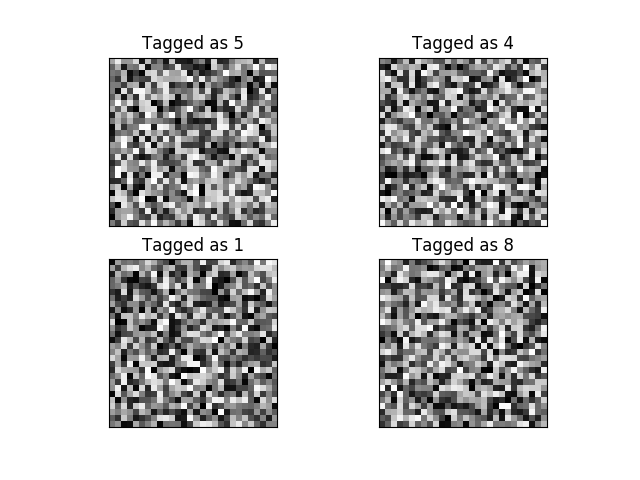
\includegraphics[width=\linewidth]{../data/wm.png}
     \caption{Water marks images.}
  \end{subfigure}
  \begin{subfigure}{0.4\linewidth}
    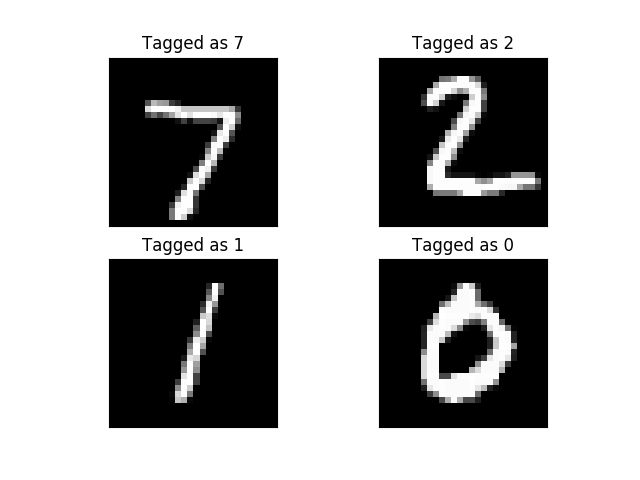
\includegraphics[width=\linewidth]{../data/mnist.png}
    \caption{MNIST images.}
  \end{subfigure}
  
  \label{fig:Image examples}
\end{figure}
The first test we did was to find the minimal change according to $\norm{\cdot}_{\infty}$ norm and $\norm{\cdot}_1$ norm for every water mark image 

\section{Related Work}
\label{sec:relatedWork}

\section{Conclusion and Future Work}
\label{sec:conclusion}


\bibliographystyle{abbrv}
\bibliography{watermarks}

\end{document}

%%% Local Variables:
%%% mode: latex
%%% TeX-master: t
%%% End:
